\documentclass[runningheads]{llncs}
\usepackage{graphicx}
\usepackage[width=122mm,left=12mm,paperwidth=146mm,height=193mm,top=12mm,paperheight=217mm]{geometry}
\usepackage{amsmath,amssymb} % define this before the line numbering.

\DeclareMathOperator*{\argmin}{argmin}

%\usepackage{ruler}
\usepackage{color}

%\documentclass{llncs}
%\usepackage{graphicx}
%\usepackage{geometry}
%\geometry{margin=2cm}
%\usepackage{amsmath}

\usepackage{pgfplots}
\usepackage{filecontents}
\usepackage[caption=false]{subfig}
\usepackage{listings}
\lstset{
basicstyle=\small\ttfamily,
columns=flexible,
breaklines=true
}

\begin{document}
\title{Dissecting Neural Style Transfer}
\author{Xi Du}
\institute{Australian National University, Australia\\
\email{u6559090@anu.edu.au}}
\maketitle 
\begin{abstract}
\cite{method}

\keywords{Neural network, Deep learning, 
Small data, Interpretability .}
\end{abstract}

\section{Introduction}

Image stylization is the process that mimics the appeal of artistic media [1] and converts input images into a stylized version. It is a research started with semi-automatic painting systems since 1990s [2] and can be used in many newly developed applications in machine learning and artificial intelligence [3]. This technique leads to a new form of communication [4]. With the use of image stylization, the media users can keep stylistic consistency on media platforms like Instagram or Twitter without obtaining skills in traditional artistic techniques [5]. Image stylization allows users to generate picture in traditional artistic styles, which had been expensive and time-consuming with traditional techniques [19]. It shifts the way how the media users share pictures on internet. At the beginning of the image stylization, which it started in 1980s, procedural filters and patch-based algorithms were studied and applied [4]. One example for the procedural filters is to refine image with strokes placement algorithms, which a grid of rendering brush strokes is placed over an image [12, 13]. Later on, patch-based synthesis was studied based on texture recognition [14]. Moreover, these two methods have numerous difficulties in further developments on the capture of complex nuances of an artist’s style, and can only work for certain types of images [4]. However, deep neural networks, which are developed as a general-purpose tool working different computer vision problems [15].  The paper published by Leon Gatys in 2015 has proven that a simple neural network works well on the texture recognition just like the patch-based synthesis algorithms [16]. 
One of the applications is auto-painter for cartoon image generation and it applies deep neural networks on image stylization [7]. These computational bio-inspired neural networks mimic the basic structure of brain neurons. Like the auto-painter, convolutional neural network is used in this paper for developing a tool in image stylization. Neural networks, especially for the deep artificial neural networks, has been widely studied and used in the pattern recognition and machine learning in recent years [8]. Convolutional neural network is one of the deep learning neural networks and have substantially achieved the state-of-the-art accuracies of object recognition [11]. This is the key in image stylization where the essential features in the style image are extracted and applied on the input image. 
This paper applies a pre-trained CNN, VGG-19, on image stylization and extends its possibilities on image stylization. CNNs have a similar structure as ordinary neural networks, which include neurons with learnable weights and biases. CNNs are typically feed-forward architecture and widely used in computer vision tasks in recent years [11]. Its basic unit is single neuron. Each of these neurons takes one or multiple inputs, conducts a dot product then optimally follows it with a non-linearity [9]. The core mathematical equation for CNN is a result derived from two functions by integration and this indicates how one’s shape is changed by the other. CNN works in a way similar to broad categorization [10]. When a CNN is used in image processing, every pixel of the input image will be processed by a feature detector and a feature map is given as the result. There will be very less, but critical features kept in the feature map compared to the input image. Consequently, some key features might be missed, and massive trainings are required for CNN’s accuracy on texture capture. 

\section{Related Work}



\section{Method}

\subsection{Deep Neural Network}

For the purpose of implementing and even extending neural style transfer algorithms,
it is not necessary to understand how a neural network is trained, because
we can use pretrained model for example vgg19 \cite{vgg19}.

It is necessary to point out that a deep neural network that neural style transfer
is concerend about
is just a sequence of functions
$F_1,F_2,F_3,...$
whose inputs and outputs are all multi-dimensional arrays, as illustrated in Figure \ref{f1f2f3}.
\begin{figure}
\center
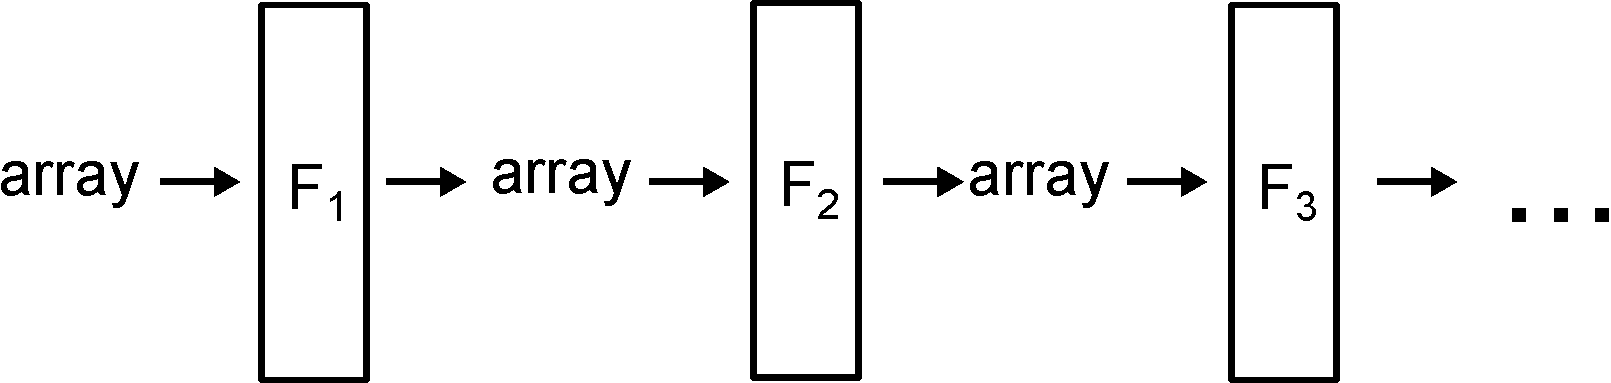
\includegraphics[width=0.6\textwidth]{f1f2f3.pdf}
\caption{A deep neural network \label{f1f2f3}}
\end{figure}
Because the arrays have usually more than two numbers of dimensions
they are not really matrices.
The arrays are called tensors (as in TensorFlow or torch.Tensor in PyTorch) 
but actual tensor algebra in a mathematical sense is rarely relevant.
The functions need to be differentiable, which is handled automatically by modern 
deep learning frameworks.
Other than that we can treat the functions as blackboxes because we are 
not concerned of training the model.
A ``layer'' in a deep neural network refers to a few consecutive functions together.
It is not particularly necessary to consider ``layers'' in this work. 
Though it is important to note that in our illustrations there are functions instead of layers.

\subsection{vgg19 model}
For the vgg19 model that most neural style transfer implementations available are based on,
The inputs and outpus of each function are all arrays with 4 dimensions.
The word ``dimension'' here may mean something slightly different from what ``dimension'' means in
for example ``$3$-dimension vector''. 
Some people call the number of dimensions ``rank'' which would then raise another confusion with the rank of matrices.
We give an illustration for the vgg19 model in Figure \ref{vgg512}
\begin{figure}
\center
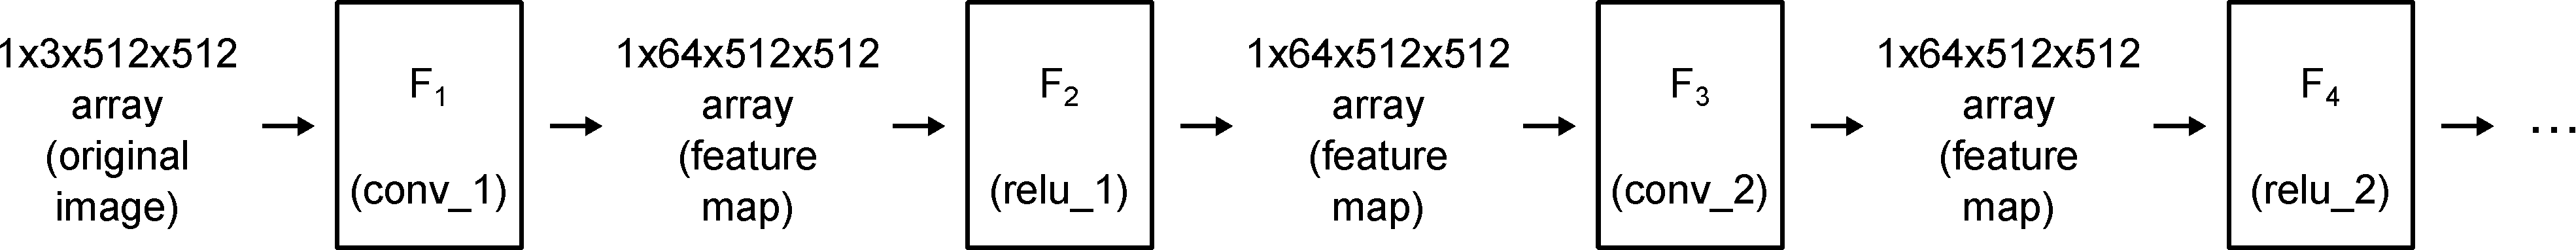
\includegraphics[width=\textwidth]{vgg512.pdf}
\caption{The VGG19 model with an $512\times512$ RGB image as its input \label{vgg512}}
\end{figure}

The 1st dimension is the ``batch'' dimension, which means that you can put several images through the
series of functions.
In neural style transfer implementations it is usually just one image each time.
So the 1st dimension is always 1, even between the $F$ functions, throughout this work.

The 2nd dimension is the ``feature'' dimension. For a raw RGB image, it is 3.
Intermediate arrays between, for example, $F_3$ and $F_4$, usually 
have a size much larger than 3, such as 64 or 128.

The 3nd and 4th dimensions are just spatial locations. 
For a $512\times512$ image they are 512 and 512. 
For intermediate arrays, these 2 dimensions are sometimes scaled down
to half or even $\frac{1}{4}$ of the sizes of the image.

The functions $F_1,F_2,F_3,...$ now have meaningful names such as relu\_1, conv\_2 now.
[[[[Not actually necessary to know but insert your elaborations here]]]]

The arrays after the initial image are called \emph{feature maps}, because their value means
``how much a feature x exists at position y and x''.
Take a $1\times64\times512\times512$ feature map for example. There are 64 types of features.
Its [1, 17, 111, 222] element, would then refer to the extent that the 17th type feature exists
at the position of the 222th column of the 111th row. This ``extent'' could also be negative.

\subsection{Vanilla neural style transfer}

The vanillay neural style transfer algorithm \cite{nst} is 
structured as iteratively solving an optimisation problem.
The argument to optimise is the image as a multidimensional array,
of size $1\times3\times512\times512$ for example.
The interative solver can be many, but in our case it is 
L-BFGS [[[[Maybe elaborate on L-BFGS here]]]]. 
The initial value of the argument could be either white noise or the content image,
but the latter appeared to make the optimisation much easier.

The key issue here is still how to structure the optimisation target.
The value to minimise is a linear combination of a ``style loss'' 
and ``content loss''.
Although these appeared to be two weights,
actually only their ratio mattered.
We simply fixed the weight of the content loss to 1 and
leave the weight of the style loss as a adjustable hyperparameter $k$.
\begin{align}
\argmin\limits_{\text{image}} (kL_\text{style}+L_\text{content})
\end{align}

The content loss $L_\text{content}$ is the easier one to explain of the two losses.
It is the mean square error between the outputs of a certain function in the
vgg19 taking the current argument image and the content image as inputs respectively.
We say ``a certain'' function because the output of which function to choose is
adjustable.
A typical choice is the output of \verb|conv_4| function. See Figure \ref{contentloss}.
\begin{figure}
\center
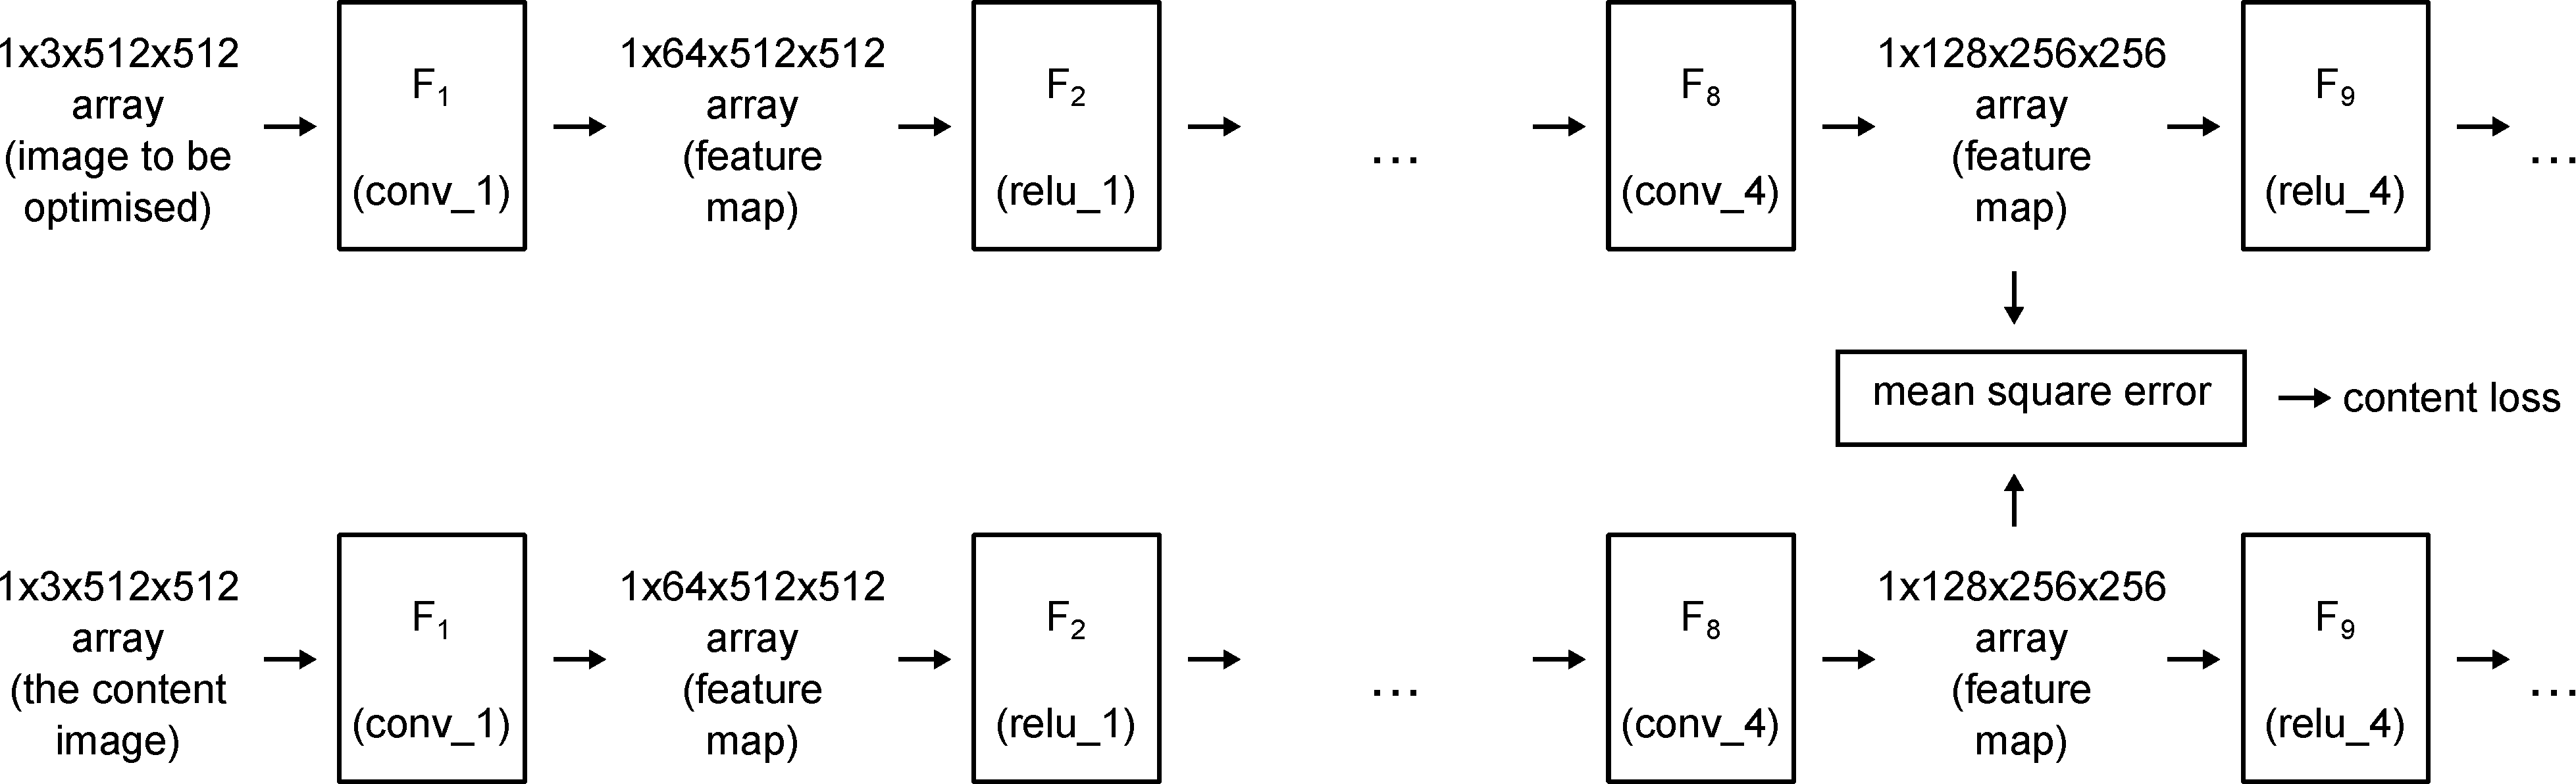
\includegraphics[width=\textwidth]{contentloss.pdf}
\caption{The content loss \label{contentloss}}
\end{figure}


The style loss $L_\text{content}$ can actually be a sum of several style losses, or sometimes just one.
For each style loss, 
both the current image under optimisation and the style image are passed through the vgg19 model.
The two outputs of a certain function in the model are extracted, 
and converted to Gram matrices. We will elabrate on what Gram matrices are later.
For now a Gram matrix is just a square matrix computed from a multidimensional array (i.e. a feature map).
For example, the Gram matrix (in the style transfer algorithm) of a $1\times64\times512\times512$ array
is a $64\times64$ matrix.
The point is that a Gram matrix describes the distribution of features
in the image without the spatial information of where the features are.
Gram matrices describe the distribution with correlation between features.
The several style losses are computed with the outputs of different functions.
Otherwise, each of the several style losses are computed in exactly the same way.
Again, the outputs of which functions in the model to derive style losses from is really adjustable.
A nice default we used was \verb|conv_1|,\verb|conv_2|,...,\verb|conv_5|. We illustrate
the style losses derived from the output of \verb|conv_1| in Figure $\ref{styleloss}$.

\begin{figure}
\center
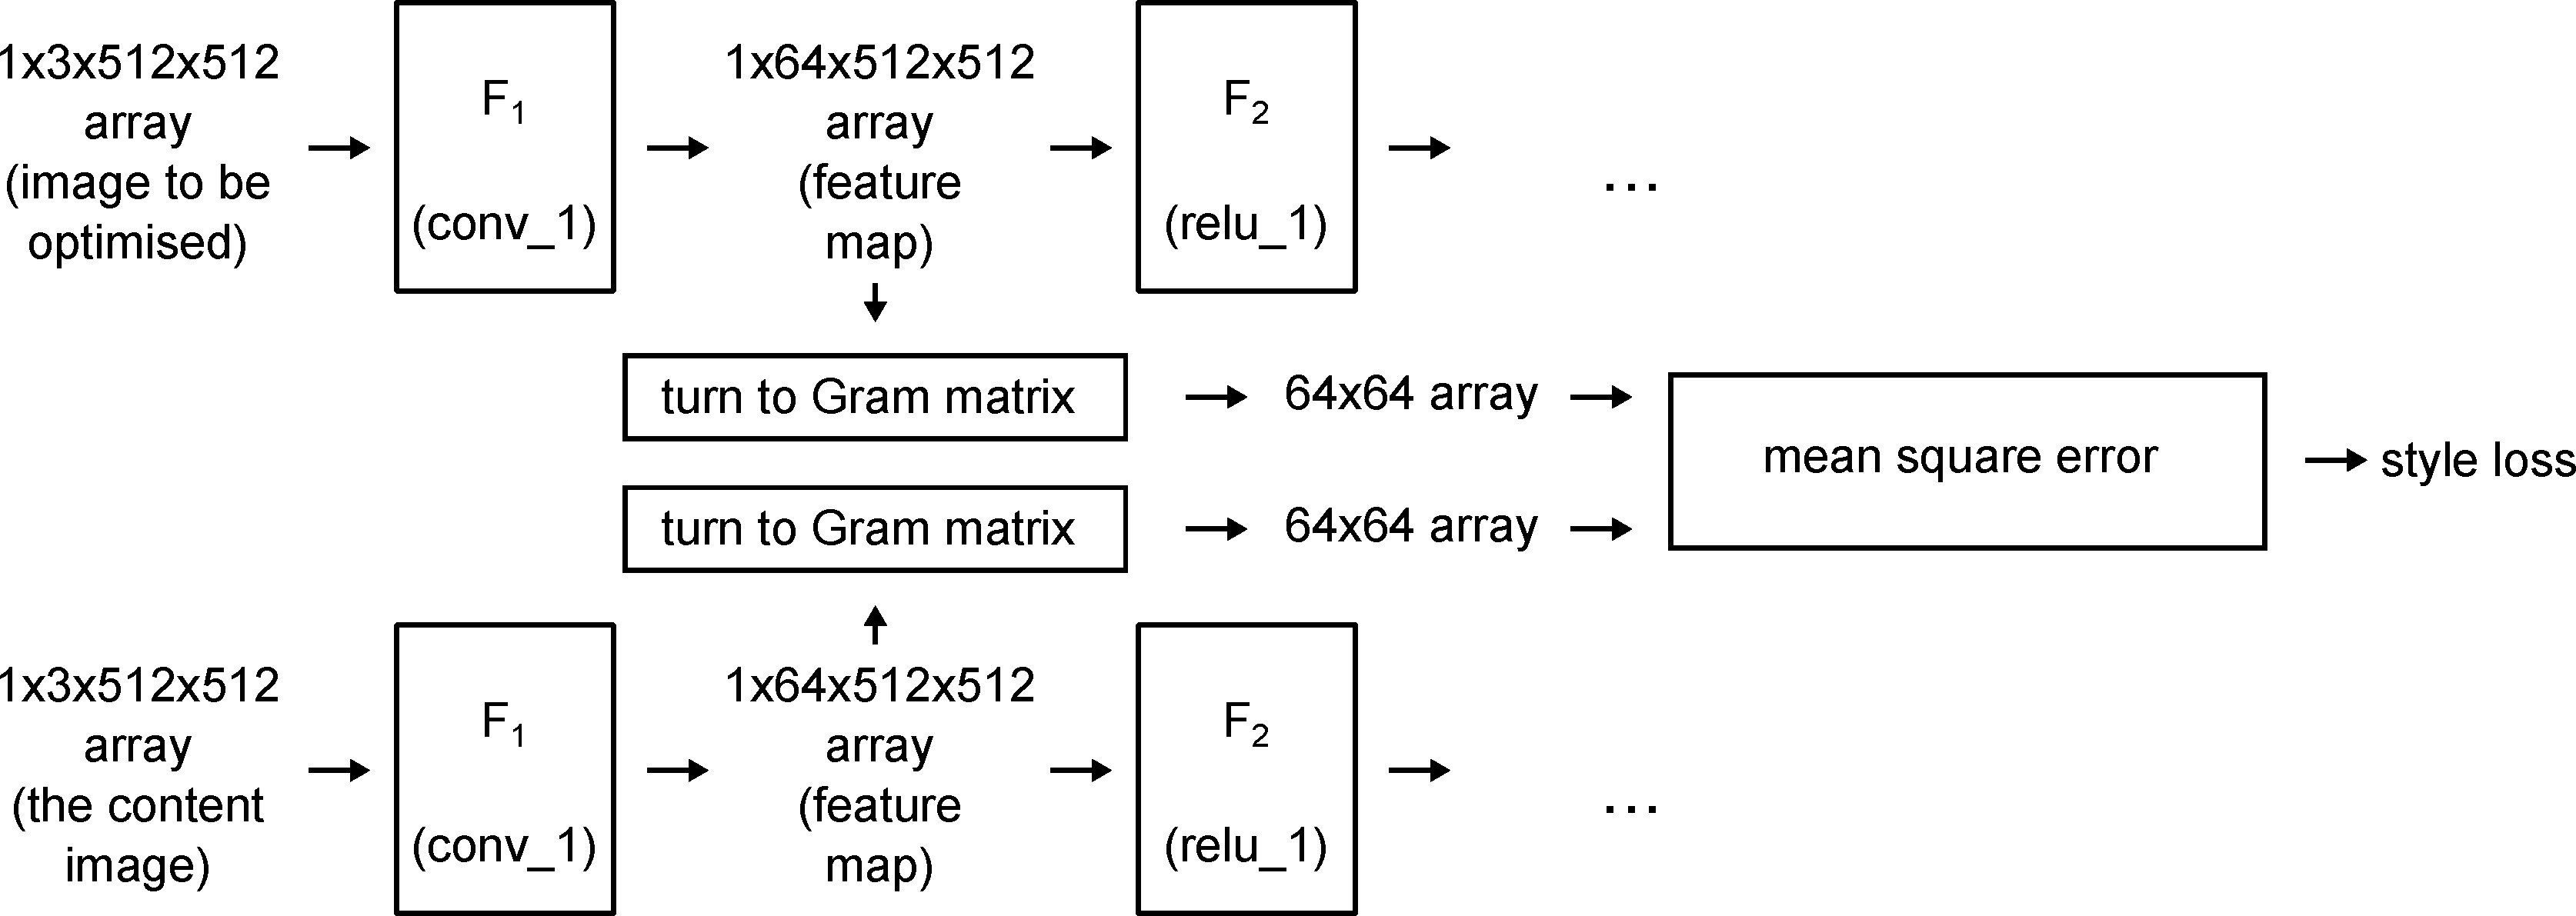
\includegraphics[width=\textwidth]{styleloss.pdf}
\caption{The style loss derived from the output of conv\_1 \label{styleloss}}
\end{figure}

\subsection{Gram matrix}
[[[[Elaborate on gram matrix here]]]]

\subsection{Removing the spatial information in other ways}
We think that the most brilliant aspect of the neural style transfer algorithm,
apart from the general structure, is the use of Gram matrices to compare 
distributions of features in two images, so that where the features are does not matter.
It gives really nice insight on what ``artistic style'' means.

Now we wonder, could we achieve similar results with other ways to compare 
distribution of features?
One approach would be to consider the \emph{comparison} as a whole to find 
substitutes. 
For example, minimising the mean square errors between two Gram matrices could be seen as 
a special case for minimising a Maximum Mean Discrepancy (MMD), which means other Maximum Mean Discrepacies
could be used \cite{MMD}.

[[[[Maybe Describe MMD here]]]]

For us, it seemed more natural to consider substitutes for the process itself of 
transforming a feature map into a Gram matrix. 
That is, we will consider other
mappings that remove the spatial information or where features are in a feature map but retain
the distribution of features, like a histogram.
Such functions need to be differentiable as well, otherwise they would render the 
optimisation infeasible.

We will call such functions ``\emph{dislocators}'' in the remaing part of this work.
Unfortunately, the word ``dislocate'' would give the connotation of moving something to somewhere else.
Nevertheless, the word ``locator'' means something that provides spatial information,
so calling somthing that removes spatial information a ``dislocator'' is still reasonable.

Other ``dislocator'' functions whose output somehow describe the 
distribution of features in their input should then work as substitutes
for computing Gram matrices.
The first few simplistic ``dislocator'' functions we tried are listed here.
\begin{enumerate}
\item Scaled sum of the responses all over the place for each feature.
That is, for an $1\times64\times256\times256$ feature map,
we compute an $1\times64$ array where each element is the sum of the
$256\times256$ elements from the input.
The whole array is then scaled to one over the total number of elements of the input feature map.
\item Scaled sum of element-wise squares of the responses over the place for each feature.
Other than an additional element-wise squaring, it is identical to the previous one.
\item Scaled sum of absolute values of the responses over the place for each feature.
\end{enumerate}

To find more dislocators, let us consider \emph{how to describe a distribution} in general?
The obvious answer is then sample statistics or estimators, like (sample) mean, (sample) standard deviation, 
(sample) skewness, (sample) kurtosis and any moments.
Unfortunately, we found that higher moments too slow to compute for our experiments,
so we ended up with the following (combinations) of sample statistics.
\begin{enumerate}
\item Mean and standard deviation of each type of feature. 
That is, given a $1\times64\times256\times256$ feature map, 
we compute an $1\times64\times2$ array.
Standard deviation is favored over variance because standard deviations 
are supposedly of the same unit of measure as the mean, 
while variances are of a squared unit of measure.
\item Mean, standard deviation and 4th central moment to the power of $1/4$. 
That is, a $1\times64\times3$ array for a $1\times64\times256\times256$ feature map.
\item Mean, standard deviation, 4th central moment to the power of $1/4$, 
and 6th central moment to the power of $1/6$.
\end{enumerate}
We have found by experiment that odd-order moments did not work.
6th central moments were already much slower to compute in practice 
than Gram matrices.
So we could only stop at the 6th moment due to limited experimental capacity.

Unfortunately, straight forward histograms were not computationally feasible.
Although the autograd facility could handle histograms in theory, we were not
able to make histograms work in practice. Similarly, sorting or order statistics
like medians were found to be computationally infeasible in practice.

\section{Experiments and Discussion}

\subsection{Reproducing the original result}
[[[[Fill the experiment part in demo here to show that we have reproduced result.
Cite the original tutorial]]]] \cite{tut}

\subsection{Varying the extraction points for losses}

We will now show that within the general optimisation framework,
steps other than the Gram matrix, 
such as the outputs of which feature maps to derive the style 
losses from are not very essential.

\subsection{Varying the dislocator function}

Now let us see something more interesting.


\section{Conclusion and Future Work}

\begin{thebibliography}{8}
\bibitem{nst}
Gatys, L., Ecker, A., \& Bethge, M. (2016). A neural algorithm of artistic style. Journal of Vision, 16(12), 326. doi:10.1167/16.12.326
\bibitem{MMD}
Li, Y., Wang, N., Liu, J., \& Hou, X. (2017). Demystifying Neural Style Transfer. IJCAI.
\bibitem{interp}
Doshi-Velez, F., \& Kim, B. (2017). Towards A Rigorous Science of Interpretable Machine Learning.
\bibitem{pytorch}
Paszke, A., Gross, S., Chintala, S., Chanan, G., Yang, E., DeVito, Z., Lin, Z., Desmaison, A., Antiga, L., \& Lerer, A. (2017). Automatic differentiation in PyTorch.
\bibitem{tut}
Jacq, A. (n.d.). Neural Transfer Using PyTorch (W. Herring, Ed.). Retrieved from https://pytorch.org/tutorials/advanced/neural\_style\_tutorial.html
\end{thebibliography}
\end{document}

